\section{Sessions}

\subsection{Research Sessions}

% \begin{frame} %hmm.. thought i could change colour here :S
% \frametitle{Social Networks and Graph Databases}
% 
% \begin{itemize}
% \item A Model-Based Approach to Attributed Graph Clustering	
% 
% Zhiqiang Xu, Yiping Ke, Yi Wang, Hong Cheng, James Cheng, 	
% \item Towards Effective Partition Management for Large Graphs	
% 
% Shengqi Yang, Xifeng Yan, Bo Zong, Arijit Khan (University of California, Santa Barbara)
% \item TreeSpan: Efficiently Computing Similarity All-Matching	
% 
% Gaoping Zhu, Xuemin Lin,  Ke Zhu,  Wenjie Zhang (University of New South Wales), Jeffrey Xu Yu, (CUHK)
% \end{itemize}
% 
% \end{frame}
% 
% \begin{frame} %hmm.. thought i could change colour here :S
% \frametitle{A Model-Based Approach to Attributed Graph Clustering	}
% 
% Zhiqiang Xu, Nanyang Technological University; Yiping Ke, Institute of High Performance Computing, Singapore; Yi Wang, National University of Singapore; Hong Cheng, The Chinese University of Hong Kong; James Cheng, Nanyang Technological University	
% 
% \end{frame}
% 
% \begin{frame} %hmm.. thought i could change colour here :S
% \frametitle{Towards Effective Partition Management for Large Graphs}
% 
% 
% Sledge
% adjust partitions to serve queries efficiently
% 
% Done: dynamic graph partitioning. overlap graph partitioning (Parrallel dynamic graph partitioning for adaptive unstructured meshes (PDC 1997)
% 
% Contribution: dynamic workload adaptive (dynamic) graph partitioning
% \end{frame}
% 
% \begin{frame} %hmm.. thought i could change colour here :S
% \frametitle{TreeSpan: Efficiently Computing Similarity All-Matching}
% 
% %     \begin{figure}
%     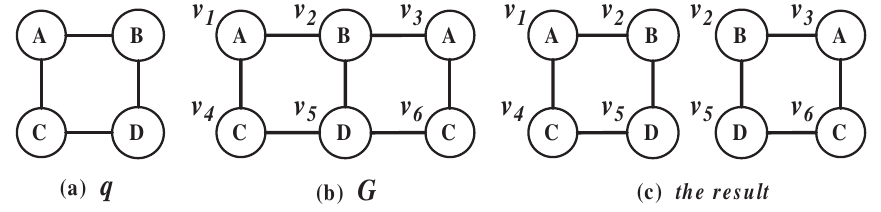
\includegraphics[width=0.85\textwidth]{images/SNGD-3-0.png} 
% %     \end{figure}
% 
% \begin{itemize}
% \item sub-graph containment
% \item graph indexing
% \item SAPPER: Subgraph indexing and approximate matching in large graphs (VLDB 2010)
% \end{itemize}
% 
% \end{frame}
% 
% 
% \begin{frame} %hmm.. thought i could change colour here :S
% \frametitle{TreeSpan: Efficiently Computing Similarity All-Matching}
% 
% Find similarity all-matching up to a $\theta$ threshold ($\theta = 2$ used  in figures)
% 
% Compute all maximal matches (spanning trees) 
% 
%     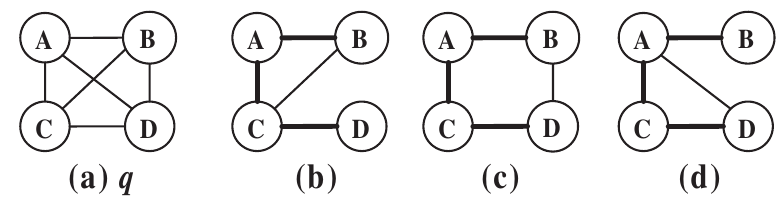
\includegraphics[width=0.80\textwidth]{images/SNGD-3-1.png} 
%  
% 
% \end{frame}
% 
% \begin{frame} %hmm.. thought i could change colour here :S
% \frametitle{TreeSpan: Efficiently Computing Similarity All-Matching}
% 
% 
% 
%     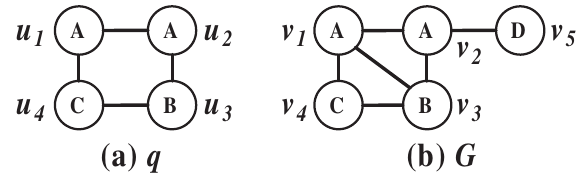
\includegraphics[width=0.75\textwidth]{images/SNGD-3-2.png} 
% 
%     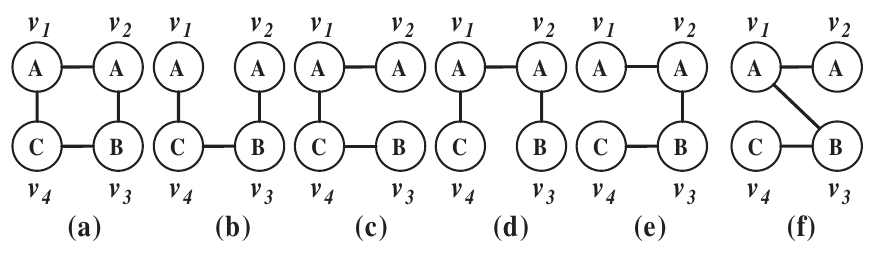
\includegraphics[width=0.75\textwidth]{images/SNGD-3-3.png} 
% 
% \end{frame}
% 
% \begin{frame} %hmm.. thought i could change colour here :S
% \frametitle{TreeSpan: Efficiently Computing Similarity All-Matching}
% 
% 
% 
%     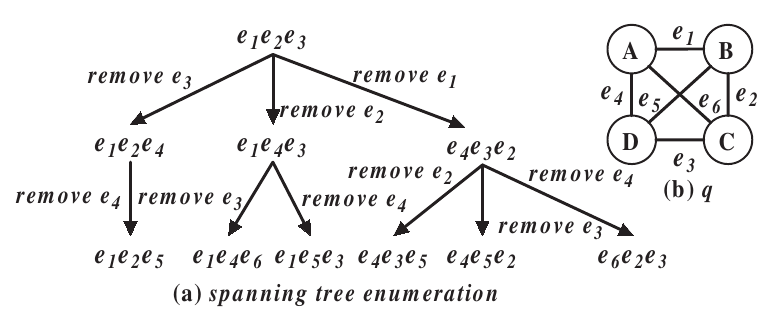
\includegraphics[width=0.75\textwidth]{images/SNGD-3-4.png} 
% 
%     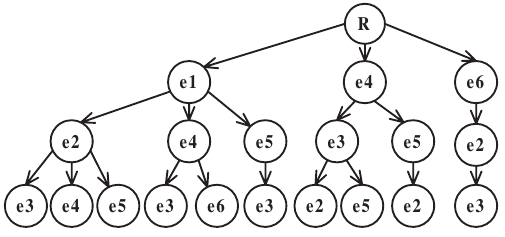
\includegraphics[width=0.75\textwidth]{images/SNGD-3-5.png} 
% 
% \end{frame}
% 
% 
% \begin{frame} %hmm.. thought i could change colour here :S
% \frametitle{Temporal and Graph Databases}
% \begin{itemize}
% \item Temporal Alignment
% 	
% Anton Dignös, University of Zürich; Michael H. Böhlen, University of Zürich; Johann Gamper, Free University of Bozen-Bolzano
% \item A Highway-Centric Labeling Approach for Answering Distance Queries on Large Sparse Graphs	
% 
% Ruoming Jin, Kent State University; Ning Ruan, Kent State University; Yang Xiang, Ohio State University; Victor Lee, Kent State University	
% \item Efficient Processing of Distance Queries in Large Graphs: A Vertex Cover Approach
% 
% James Cheng, Nanyang Technological University; Yiping Ke, Institute of High Performance Computing, Singapore; Shumo Chu, Nanyang Technological University; Carter Cheng, Nanyang Technological University	
% 
% \end{itemize}
% 
% \end{frame}
% 
% \begin{frame} %hmm.. thought i could change colour here :S
% \frametitle{Temporal Alignment}
% 	
% Anton Dignös, University of Zürich; Michael H. Böhlen, University of Zürich; Johann Gamper, Free University of Bozen-Bolzano
% 
% \end{frame}
% 
% \begin{frame} %hmm.. thought i could change colour here :S
% \frametitle{A Highway-Centric Labeling Approach for Answering Distance Queries on Large Sparse Graphs	}
% 
% 
% Ruoming Jin, Kent State University; Ning Ruan, Kent State University; Yang Xiang, Ohio State University; Victor Lee, Kent State University	
% 
% \end{frame}
% 
% \begin{frame} %hmm.. thought i could change colour here :S
% \frametitle{Efficient Processing of Distance Queries in Large Graphs: A Vertex Cover Approach}
% 
% 
% James Cheng, Nanyang Technological University; Yiping Ke, Institute of High Performance Computing, Singapore; Shumo Chu, Nanyang Technological University; Carter Cheng, Nanyang Technological University	
% 
% \end{frame}
% 
% \begin{frame} %hmm.. thought i could change colour here :S
% \frametitle{Mobile Databases}
% \begin{itemize}
% \item MaskIt: Privately Releasing User Context Streams for Personalized Mobile Applications
% 	
% Michaela Goetz, Twitter; Suman Nath, Microsoft Research; Johannes Gehrke, Cornell University	
% \item Authenticating Location-Based Services without Compromising Location Privacy	
% 
% Haibo Hu, Hong Kong Baptist University; Jianliang Xu, Hong Kong Baptist University; Qian Chen, Hong Kong Baptist University; Ziwei Yang, Hong Kong Baptist University	
% \item Effective Caching of Shortest Paths for Location-Based Services
% 
% Jeppe Rishede Thomsen, Hong Kong Polytechnic University; Man Lung Yiu, Hong Kong Polytechnic University; Christian S. Jensen, Aarhus University	
% \end{itemize}
% 
% \end{frame}
% 
% \begin{frame} %hmm.. thought i could change colour here :S
% \frametitle{MaskIt: Privately Releasing User Context Streams for Personalized Mobile Applications}
% 
% Michaela Goetz, Twitter; Suman Nath, Microsoft Research; Johannes Gehrke, Cornell University	
% 
% \end{frame}
% 
% \begin{frame} %hmm.. thought i could change colour here :S
% \frametitle{Authenticating Location-Based Services without Compromising Location Privacy}
% 
% 
% Haibo Hu, Hong Kong Baptist University; Jianliang Xu, Hong Kong Baptist University; Qian Chen, Hong Kong Baptist University; Ziwei Yang, Hong Kong Baptist University	
% 
% \end{frame}
% 
% \begin{frame} %hmm.. thought i could change colour here :S
% \frametitle{Effective Caching of Shortest Paths for Location-Based Services}
% 	
% 
% Jeppe Rishede Thomsen, Hong Kong Polytechnic University; Man Lung Yiu, Hong Kong Polytechnic University; Christian S. Jensen, Aarhus University	
% \end{frame}


\begin{frame} %hmm.. thought i could change colour here :S
\frametitle{Distributed and Parallel Databases}
\begin{itemize}
\item Calvin: Fast Distributed Transactions for Partitioned Database Systems	
\ritem Alexander Thomson,  Thaddeus Diamond,  Shu-Chun Weng,  Kun Ren,  Philip Shao,  Daniel J. Abadi (Yale University)

\item Advanced Partitioning Techniques for Massively Distributed Computation	
\ritem Jingren Zhou,  Nicolás Bruno,  Wei Lin (Microsoft)

\item SkewTune: Mitigating Skew in MapReduce Applications	
\ritem YongChul Kwon, Magdalena Balazinska, Bill Howe (University of Washington); Jerome Rolia (HP Labs)
\end{itemize}

\end{frame}

\begin{frame}[plain] %hmm.. thought i could change colour here :S
\frametitle{Calvin: Fast Distributed Transactions for Partitioned Database Systems}

How do we provide fast transactions in a distributed database?

\vspace{1em} 

Issues:
\begin{itemize}
\item Several Popular distributed databases provide no transactional support (CouchDB, Cassandra, Amazon Dynamo)
\item Some distributed databases limit transactions to subsets of data (Azure, Oracle NoSQL, Megastore)
\end{itemize}

\vspace{1em}

Reasons:
\begin{itemize}
\item Reducing transactional support greatly simplifies implementation of a distributed database
\item Ensuring ACID properties on queries over several partitions incur several network round trips
\item For \textit{embarrassingly partitionable} datasets it works very well
\end{itemize}


\end{frame}

\begin{frame}[plain] %hmm.. thought i could change colour here :S
\frametitle{Calvin: Fast Distributed Transactions for Partitioned Database Systems}


For datasets with dependencies, users need to implement and ensure ACID properties in the application
\begin{itemize}
\item Slow development
\item Complex code
\item Poor performance
\end{itemize}

\vspace{1em}

Calvin enables fast transactions over multiple partitions:
\begin{itemize}
\item Runs next to a non-transactional database system
\item Precalculates a deterministic query plan before executing a query
\item Enables near-liniar scalable shared nothing DB, providing full ACID transactions
\item Node failures do not cause transactions to abort (deterministic query plan - either execute instructions later, or run on parallel replica)
\end{itemize}

\end{frame}



\begin{frame}[plain] %hmm.. thought i could change colour here :S
\frametitle{Advanced Partitioning Techniques for Massively Distributed Computation}


How do we most efficiently partition or repartition data in large distributed systems?

\vspace{1em}

\begin{itemize}
\item mapReduce scales well and can do concurrency too, but it forces developers to be aware of the mapReduce model
\item Other systems (SCOPE, DryadLINQ, Tenzing, Hive) provide high level descriptive languages and offer a single machine programming abstraction. 
\end{itemize}

\vspace{1em}

\begin{itemize}
\item Introduce optimized partitioning techniques (Hash-, range-, index-based)
\item Emphasis on finding good partition boundaries
\item Identify data dependencies
\item Considers physical data location
\end{itemize}

\end{frame}

\begin{frame}[plain] %hmm.. thought i could change colour here :S
\frametitle{SkewTune: Mitigating Skew in MapReduce Applications}

How do we handle skew in MapReduce systems?

\vspace{1em}

Existing solutions:
\begin{itemize}
\item User written skew resistant operators - extra burden on user, and only applies to certain operators
\item Use very fine grained partitions - imposes a lot of overhead
\item Get the complete output from an operator, sample it, then partition data before executing next operator - requires synchronization.
\end{itemize}

\vspace{1em}

Limitations on skew handling:
\begin{itemize}
\item Handles skew from uneven distribution of input data
\item Handles skew from uneven processing time of input
\item Does NOT handle uneven processing power of nodes
\end{itemize}

\end{frame}


\begin{frame}[plain] %hmm.. thought i could change colour here :S
\frametitle{SkewTune: Mitigating Skew in MapReduce Applications}

SkewTune:

\begin{itemize}
\item Replaces existing mapReduce implementation
\item Optimizes existing mapReduce programs without rewrite
\item Existing mapReduce programs still work
\item Compatible with existing pipelining optimizations  (no synchronization required.)
\item Does \textit{late skew detection}
\end{itemize}

\end{frame}



\subsection{Industry Sessions}

\begin{frame} %hmm.. thought i could change colour here :S
\frametitle{Social Media and Crowdsourcing}
\begin{itemize}
\item The Value of Social Media Data in Enterprise Applications	
\ritem Shivakumar Vaithyanathan, IBM Almaden Research Center 

\item Anatomy of a Gift Recommendation Engine Powered by Social Media	
\ritem Yannis Pavlidis, Madhusudan Mathihalli, Indrani Chakravarty, Arvind Batra, Ron Benson, Ravi Raj, Robert Yau, Mike McKiernan, Venky Harinarayan, Anand Rajaraman (@WalmartLabs)

\item Designing a Scalable Crowdsourcing Platform	
\ritem Chris Van Pelt, Alex Sorokin (CrowdFlower)
\end{itemize}

\end{frame}


\begin{frame}[plain] %hmm.. thought i could change colour here :S
\frametitle{The Value of Social Media Data in Enterprise Applications}


Problem: How can data from social media be used to create \textit{social entities}? 

\begin{itemize}
\item IBM datamines facebook and other social networks to create \textit{social entities} (companies, people, products)
\item Have gathered enough data to often be able to distinguish two entities of the same name if mentioned in some context.
\end{itemize}

\textbf{kind of unnerving!} But still only for research. 

\end{frame}

\begin{frame}[plain] %hmm.. thought i could change colour here :S
\frametitle{Anatomy of a Gift Recommendation Engine Powered by Social Media}

Wallmarts gift recommendation engine: ShopyCat.

\begin{itemize}
\item It is a facebook application
\item Lets you browse products based on what your friend might likes
\item Mines your interests, as well as letting you manually specify some.
\end{itemize}

    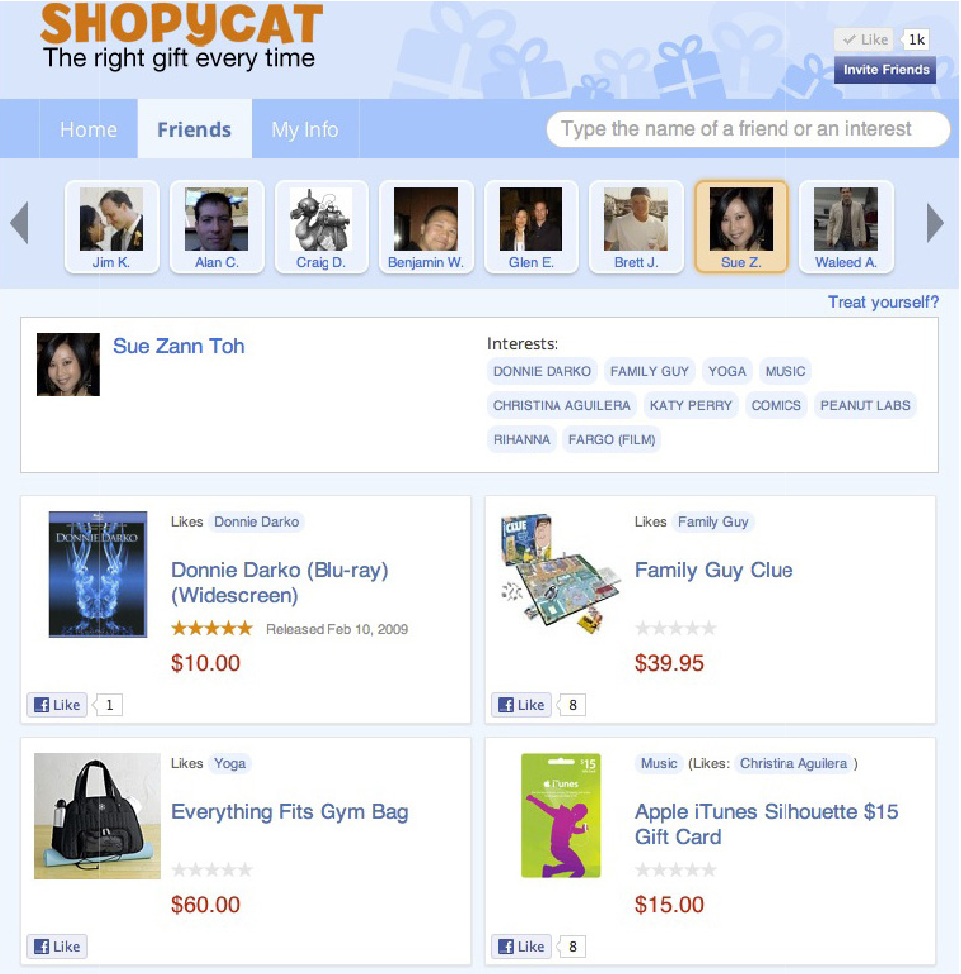
\includegraphics[width=0.5\textwidth]{images/SMC-5-1.png} 
\end{frame}

\begin{frame}[plain]
\frametitle{Anatomy of a Gift Recommendation Engine Powered by Social Media}

How to use Facebook to recommend \textit{good} gifts for users? i.e.
\begin{itemize}
\item When is it a good time to give a friend a gift? (e.g. birthday)
\item How to use friends interests to suggest specific or categories of gifts?
\item Which types of products should be available to the gift recommendation engine to cover gift categories? (from other sites than wallmart) 
\item What is a good gift in each gift category (is an item \textit{giftable}?
\end{itemize}

\vspace{0.5em}
\begin{itemize}
\ritem Several existing gift recommendation engines (Gifty, Etsy, etc.) Use semi static information (besides using likes, birthdays, life events)
\ritem ShopyCat: Only gift recommendation engine which also uses users activity 
\end{itemize}

\end{frame}


\begin{frame} [plain]%hmm.. thought i could change colour here :S
\frametitle{Designing a Scalable Crowdsourcing Platform}
	
How can we use people to solve problems that are hard for computers?

\begin{itemize}
\item CrowdFlower: a crowdsourcing platform for (many) people to solve small parts tasks 
\item Focus on 3 metrics: Quality, Cost, and Speed. Can at most do 2 at once.
\item Defines "CrowdFlower Markup Language" for task submitters to define tasks.
\item Different from competition (i.e. Mechanical Turk) in that it takes care of crowd quality for the task submitter.
\item Can use workforce from other similar services. (many very specialized such crowdsourcing services already exist)
\end{itemize}

\end{frame}




\begin{frame} %hmm.. thought i could change colour here :S
\frametitle{Modern RDBMSs} 
\begin{itemize}
\item Query Optimization in Microsoft SQL Server PDW	
\ritem Srinath Shankar,  Rimma Nehme,  Josep Aguilar-Saborit,  Andrew Chung,  Mostafa Elhemali,  Alan Halverson,  Eric Robinson,  Mahadevan Sankara Subramanian,  David DeWitt,  César Galindo-Legaria (Microsoft)

\item F1-The Fault-Tolerant Distributed RDBMS Supporting Google's Ad Business	
\ritem Jeff Shute, Mircea Oancea, Stephan Ellner, Ben Handy, Eric Rollins, Bart Samwel, Radek Vingralek, Chad Whipkey, Xin Chen, Beat Jegerlehner, Kyle Littlefield, Phoenix Tong (Google)

\item Oracle In-Database Hadoop: When MapReduce Meets RDBMS	
\ritem Xueyuan Su, Yale University; Garret Swart, Oracle 
\end{itemize}
\end{frame}



% \begin{frame} %hmm.. thought i could change colour here :S
% \frametitle{Query Optimization in Microsoft SQL Server PDW}
% 
% 
% \end{frame}
% 
% \begin{frame} %hmm.. thought i could change colour here :S
% \frametitle{F1-The Fault-Tolerant Distributed RDBMS Supporting Google's Ad Business}
% 
% 
% \end{frame}
% 
% \begin{frame} %hmm.. thought i could change colour here :S
% \frametitle{Oracle In-Database Hadoop: When MapReduce Meets RDBMS}
% 
% \textbf{Problem:} It is inefficient to make users translate their mapReduce programs if they want to take advantage of the build-in functionality in an Oracle database.
% 
%  \end{frame}


\begin{frame} [plain] %hmm.. thought i could change colour here :S
\frametitle{Oracle In-Database Hadoop: When MapReduce Meets RDBMS}

\textbf{Solution:} Implement direct support for Hadoop programs directly in Oracle DB
\begin{itemize}
\item  Source compatibility with Hadoop. users are
able to run native Hadoop applications
 
\item Access to Oracle RDBMS resident data 
 
\item Minimal dependency on the Apache Hadoop infras-
tructure. Oracle In-Database Hadoop framework
is not built on top of actual Hadoop clusters.
 
\item Greater efficiency in execution due to data pipelining,
as Oracle knows more.

\item  Seamless integration of MapReduce functionality with
Oracle SQL. 
\end{itemize}
\end{frame}











% \begin{frame}[shrink=10] %hmm.. thought i could change colour here :S
% \frametitle{Grouping} 
% 
% 
% \end{frame}
% 


